% Copyright (c) 2022 Tobias Briones. All rights reserved.
%
% SPDX-License-Identifier: CC-BY-SA-4.0
%
% This file is part of Course Project at UNAH-IS911: Microprocessors.
%
% This source code is licensed under the Creative Commons Attribution Share
% Alike 4.0 International License found in the LICENSE file in the root
% directory of this source tree or at https://spdx.org/licenses/CC-BY-SA-4.0.

\documentclass[conference]{IEEEtran}
\usepackage[letterpaper, portrait, margin=2cm]{geometry}
\usepackage[style=ieee]{biblatex}
\usepackage[utf8]{inputenc}
\usepackage[spanish]{babel}
\usepackage{geometry}
\usepackage[]{graphics}
\usepackage[demo]{graphicx}
\usepackage{csquotes}
\usepackage{float}
\usepackage{hyperref}
\usepackage[table,xcdraw]{xcolor}
\usepackage{lipsum}
\usepackage{dirtytalk}
\usepackage{listings}

\addbibresource{bibliography.bib}

\title{SENSORES Y MOTORES EN ARDUINO}
\author{
    
\includegraphics[width = 40mm]{images/logo-unah.png}\\[8ex]
    \IEEEauthorblockN{Tobias Briones}
    \IEEEauthorblockN{tobias.briones@unah.hn}
    \IEEEauthorblockA{\textit{Universidad Nacional Autónoma de Honduras} \\
    \textit{Ingeniería de Sistemas} \\
    \textit{I PAC 2022} \\
    \textit{IS911-MICROPROCESADORES}} \\\vspace*{20pt} \normalsize  \\
    \today
}

\hypersetup{
    colorlinks=true,
    linkcolor=black,
    filecolor=magenta,
    urlcolor=cyan,
    citecolor=black
}

\newcommand\blfootnote[1]{%
    \begingroup
    \renewcommand\thefootnote{}\footnote{#1}%
    \addtocounter{footnote}{-1}%
    \endgroup
}

\definecolor{codegreen}{rgb}{0,0.6,0}
\definecolor{codegray}{rgb}{0.5,0.5,0.5}
\definecolor{codepurple}{rgb}{0.58,0,0.82}
\definecolor{backcolour}{rgb}{0.95,0.95,0.92}

\lstdefinestyle{mystyle}{
    backgroundcolor=\color{backcolour},
    commentstyle=\color{codegreen},
    keywordstyle=\color{magenta},
    numberstyle=\tiny\color{codegray},
    stringstyle=\color{codepurple},
    basicstyle=\ttfamily\footnotesize,
    breakatwhitespace=false,
    breaklines=true,
    captionpos=b,
    keepspaces=true,
    numbers=left,
    numbersep=5pt,
    showspaces=false,
    showstringspaces=false,
    showtabs=false,
    tabsize=2
}

\lstset{style=mystyle}

\begin{document}

    \maketitle

    \begin{abstract}

    \end{abstract}

    \tableofcontents

    \blfootnote{
        Copyright (c) 2022 Tobias Briones. All rights reserved. \\
        This work is licensed under the Creative Commons Attribution Share Alike 4.0 International License (\href{https://spdx.org/licenses/CC-BY-SA-4.0}{CC-BY-SA-4.0}). \\
        Third party contents available under their respective copyright and license.\\
        For more details go to the \href{https://github.com/tobiasbriones/cp-unah-is911-microprocessors}{GitHub Repository}.}

    \section{Introducción}


    \section{Objetivo}

    El objetivo de esta investigación es coleccionar un marco teórico sobre sensores y motores básicos en Arduino.

    \subsection{Objetivos Específicos}

    Investigar el funcionamiento general y programas para Arduino de:

    \begin{itemize}
        \item Sensores PIR.
        \item Sensores IR.
        \item Módulo Bluetooth HC-06.
        \item Control de motores CD.
        \item Motor paso a paso unipolar.
    \end{itemize}

    \section{Sensores PIR/IR}

    Los \textbf{sensores PIR} son \textbf{sensores IR} pasivos. IR significa infrarrojo y simplemente los IR pueden emitir luz infrarroja mientras que los PIR son pasivos y solo la detectan. La \say{P} en PIR significa pasivo ya que como se dijo no emiten energía. Las aplicaciones más útiles para estos sensores destaca entre detectar cualquier objeto o persona u animal que tenga más de $5K$ de temperatura ya que estos emiten luz infrarroja que el ser humano no detecta pero el dispositivo si \cite{jost-ir-sensor-2019} y por tanto se puede saber si algo o alguien pasa o se mueve al medir un cambio diferencial en el sensor dado la energía de lo que se acerca al sensor. Todo esto se emplea para aplicaciones de seguridad por ejemplo.

    \bigbreak

    Según Wikipedia, los sensores PIR:

    \begin{quote}
        Un sensor infrarrojo pasivo (\textbf{sensor PIR}) es un sensor electrónico que mide la luz infrarroja (IR) que irradian los objetos en su campo de visión. Se utilizan con mayor frecuencia en detectores de movimiento basados en PIR. Los sensores PIR se usan comúnmente en alarmas de seguridad y aplicaciones de iluminación automática.\\
        \small Fuente: Wikipedia $\mid$ Passive infrared sensor (traducido de inglés a español) \cite{wikipedia-pir-sensor-2022}
    \end{quote}

    \begin{figure}[H]
        \centering
        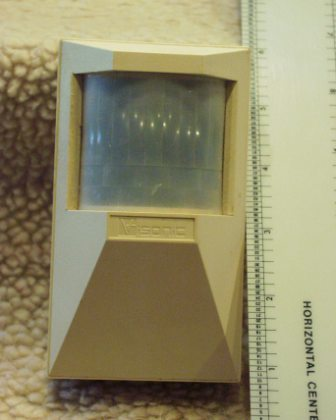
\includegraphics[width=0.2\paperwidth]{images/house-pir.jpg}
        \caption{Sensor PIR de casa}
        \footnotesize
        Fuente: Wikipedia $\mid$ Passive infrared sensor. By Jack LaRosa - Photographed and uploaded by me., Public Domain, https://commons.wikimedia.org/w/index.php?curid=4479143.
    \end{figure}

    \begin{figure}[H]
        \centering
        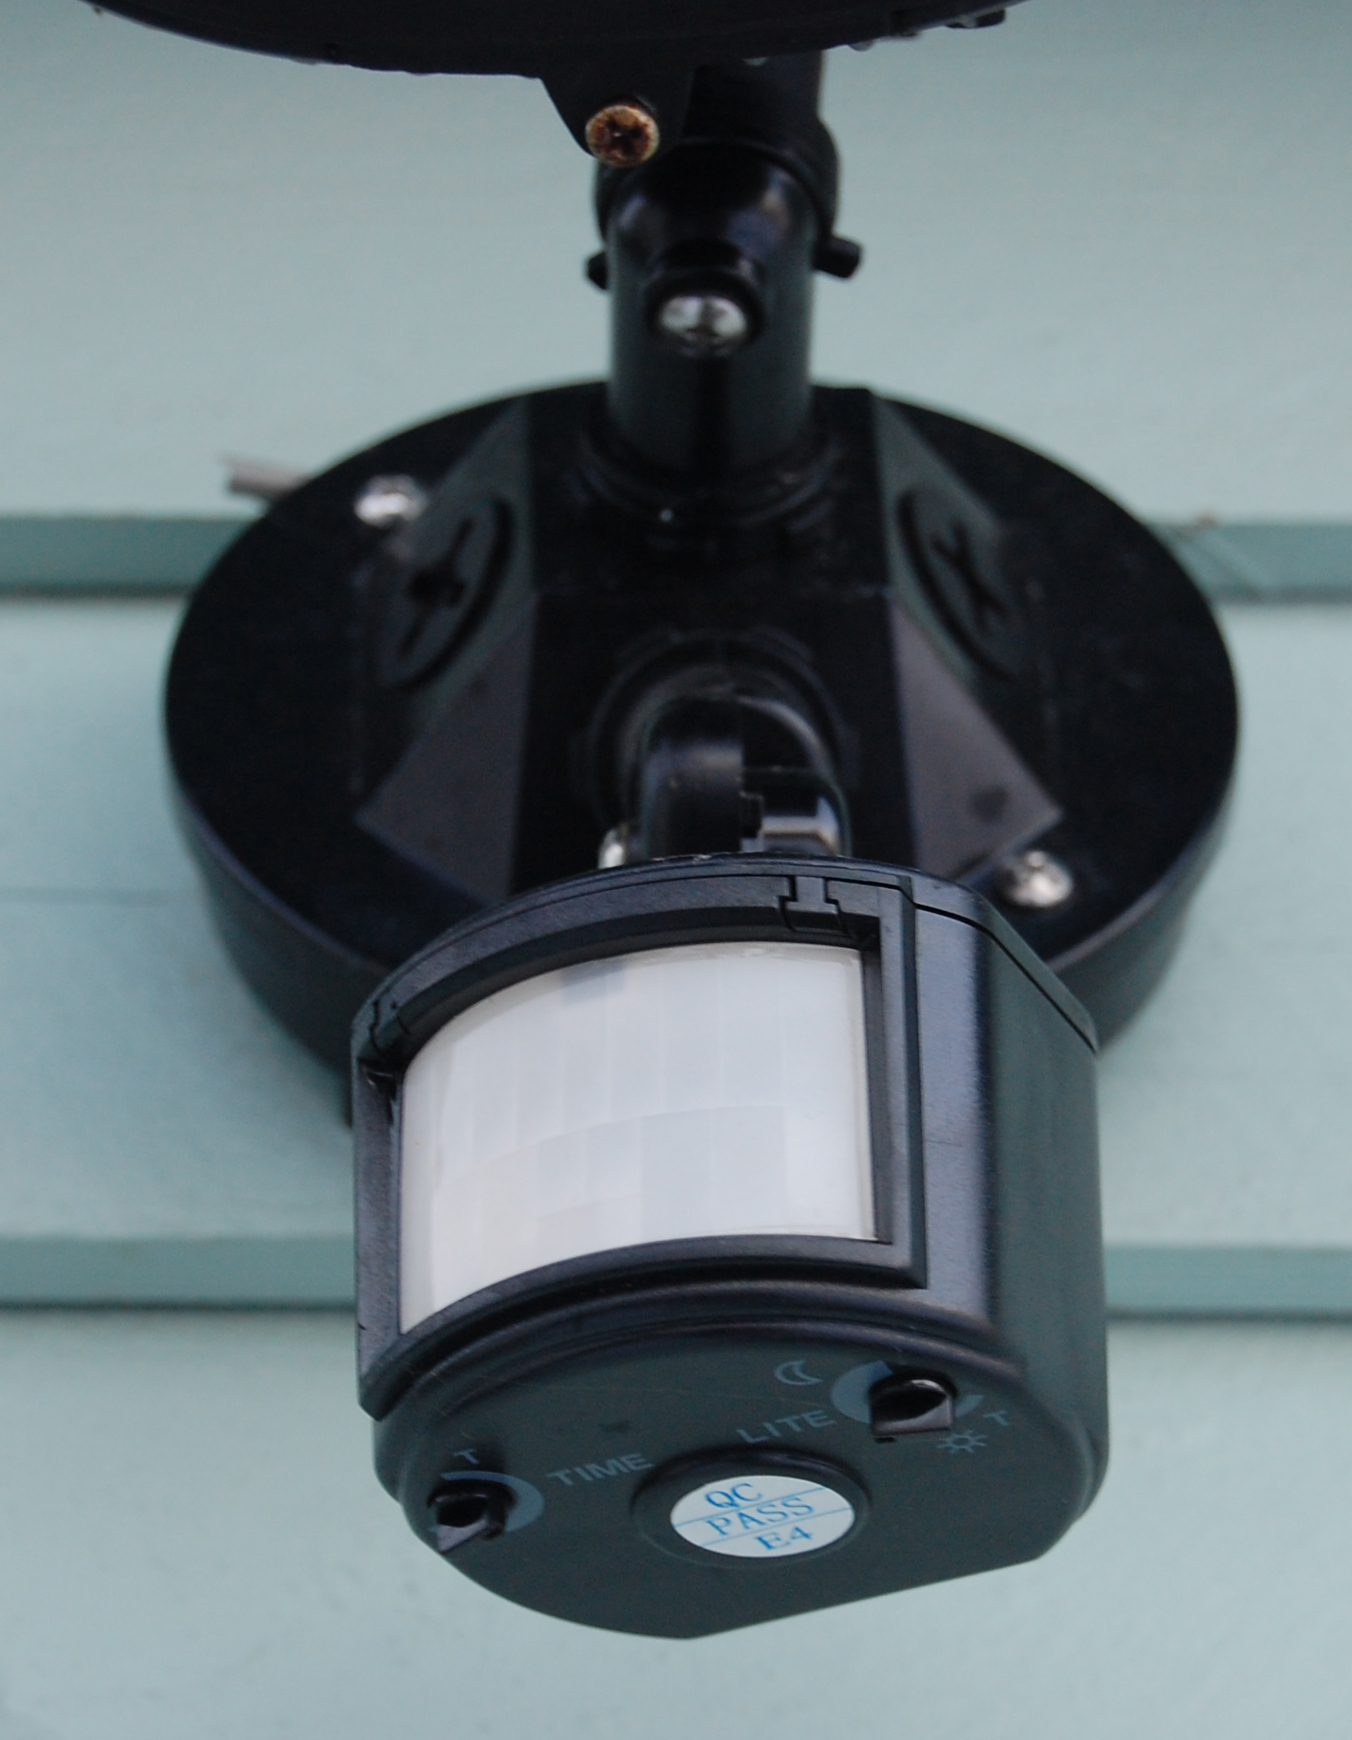
\includegraphics[width=0.2\paperwidth]{images/pir-motion-detection.jpg}
        \caption{Sensor PIR para detección de movimiento}
        \footnotesize
        Fuente: Wikipedia $\mid$ Passive infrared sensor. By CHG - Own work, Public Domain, https://commons.wikimedia.org/w/index.php?curid=6087132.
    \end{figure}

    Como se puede ver, los sensores PIR son utilizados para detección en movimiento en casas, esto puede detectar ladrones, animales, etc. Hay que tener en cuenta el lugar para la instalación de estos dispositivos para evitar falsos positivos, por ejemplo, evitar que el sensor detecte el ambiente exterior por una ventana.

    \bigbreak

    Los sensores PIR funcionan mediante la detección de un cambio en la temperatura que detectan internamente. Estos no pueden medir la temperatura pero si el cambio que se da cuando un objeto pasa por el sensor. Hay dos sensores sensibles a la luz infrarroja internamente que detectan la temperatura del ambiente y al pasar un objeto caliente a través del sensor, esa temperatura es detectada por una de las placas o sensores y estas dos señales son la entrada de un amplificador diferencial \footnote{Un amplificador operacional se puede decir que es un amplificador diferencial más sensible con más ganancia.} el cual produce la señal de cambio ya sea una cambio positivo si el objeto más caliente va pasando o negativo si va saliendo. Al no haber cuerpos calientes cercanos las señales se cancelan. \cite{wikipedia-pir-sensor-2022} \cite{adafruit-learning-system-pir-how-it-works-2014B}.

    \begin{figure}[H]
        \centering
        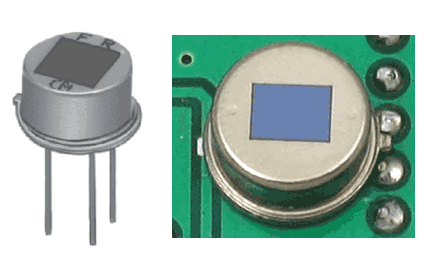
\includegraphics[width=0.2\paperwidth]{images/proximity-pyrosensor.png}
        \caption{Sensor de proximidad piroeléctrico}
        \footnotesize
        Fuente: Adafruit Learning System $\mid$ How PIRs Work. Converted from GIF to PNG. By lady ada. Licensed under the Attribution-ShareAlike Creative Commons License.
    \end{figure}

    La siguiente figura explica como funciona un PIR:

    \begin{figure}[H]
        \centering
        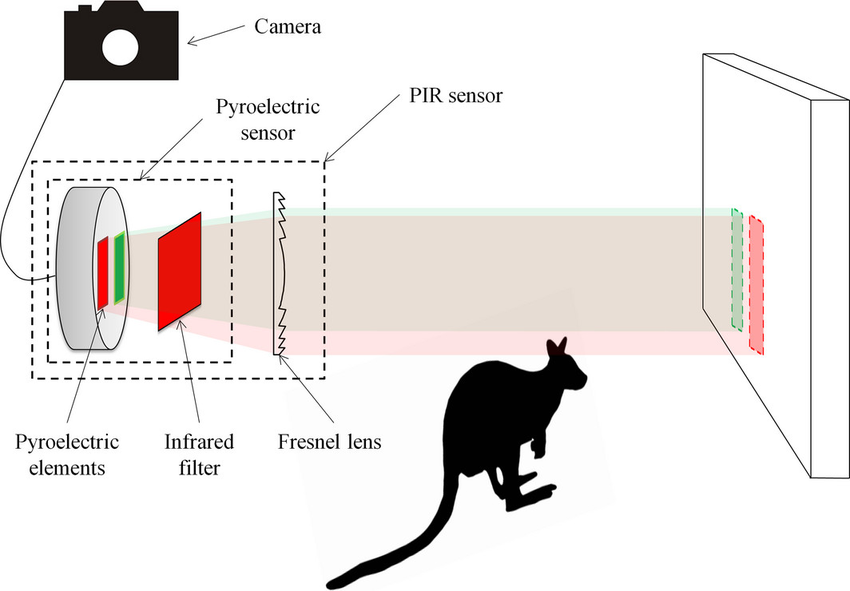
\includegraphics[width=0.3\paperwidth]{images/pir-trigger-consists-of-a-pyroelectric-sensor-and-fresnel-lens.png}
        \caption{El sensor PIR consiste de un sensor piroeléctrico y de un lente de Fresnel}
        \footnotesize
        Fuente: Research Gate $\mid$ How do passive infrared triggered camera traps operate and why does it matter? Breaking down common misconceptions. Licensed under the Creative Commons Attribution-NonCommercial 4.0 International.
    \end{figure}

    El lente de Fresnel se puede utilizar para recopilar la luz de forma más puntual y el resto del funcionamiento es como se ha descrito anteriormente.

    \subsection{Sensor PIR en Arduino}

    Este programa Arduino demuestra como utilizar el sensor PIR para detectar objetos cercanos. El sensor PIR simplemente actúa como entrada digital para establecer si hay o no hay objeto en el área de visión del sensor.

    \begin{lstlisting}[language=C, caption=Sensor PIR en Arduino. Fuente: Adafruit Learning System $\mid$ PIR Motion Sensor \cite{adafruit-learning-system-pir-sensor-2014A}]
/*
* PIR sensor tester
* by Adafruit Learning System
*/

int ledPin = 13;
int inputPin = 2;
int pirState = LOW;
int val = 0;

void setup()
{
pinMode(ledPin, OUTPUT);
pinMode(inputPin, INPUT);
Serial.begin(9600);
}

void loop()
{
val = digitalRead(inputPin);
if (val == HIGH)
{
digitalWrite(ledPin, HIGH);
if (pirState == LOW)
{
Serial.println("Motion detected!");
pirState = HIGH;
}
}
else
{
digitalWrite(ledPin, LOW);
if (pirState == HIGH)
{
Serial.println("Motion ended!");
pirState = LOW;
}
}
}
\end{lstlisting}

\bigbreak

Simplemente se definen la salida del LED en la terminal $13$ del Arduino y la entrada del sensor en el PIN $2$. Se tiene una variable de estado $pirState$ para depurar por Serial el valor actual del sensor. En la variable $val$ se guarda el valor digital del sensor.

\bigbreak

El diagrama del circuito es simplemente:

\begin{figure}[H]
\centering
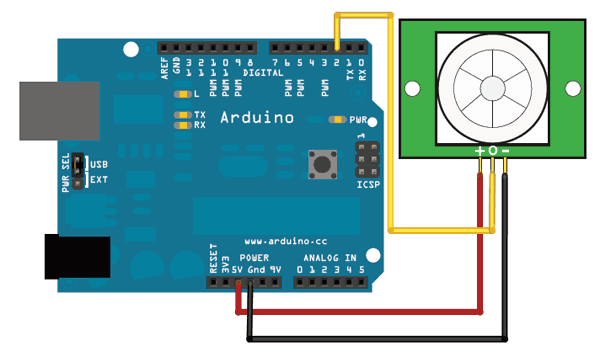
\includegraphics[width=0.3\paperwidth]{images/proximity-pir-arduino-circuit.png}
\caption{Circuito para sensor PIR en Arduino}
\footnotesize
Fuente: Adafruit Learning System $\mid$ Using a PIR w/Arduino. Converted from GIF to PNG. By lady ada. Licensed under the Attribution-ShareAlike Creative Commons License.
\end{figure}

El cual consiste en alimentar el sensor y conectar la salida del sensor a la entrada $2$ del Arduino. Recordar también conectar el LED a la terminal $13$ del Arduino.

\subsection{Sensores IR}

Los sensores IR activos actúan como sensores de proximidad al contar con la emisión de luz LED, recordando el principio de que la luz puede salir y ser reflejada por el objeto \say{intruso} y poder medir la latencia . Básicamente esa es la diferencia con respecto a los PIR.

\section{Módulo Bluetooth HC-06}

Con conectividad Bluetooth se puede tomar mayor control sobre las aplicaciones en Arduino al poder pasar el control a dispositivos móviles como smartphones. Existen dos módulos populares, el HC-06 y el HC-05 los cuales presentan diferencias principalmente en el software y con respecto a funcionalidad en tanto a que el HC-06 solo funciona como esclavo mientras que el HC-05 puede ser esclavo o maestro. Esto significa que una conexión de un esclavo solo puede conectarse a un maestro únicamente mientras que un módulo maestro no tiene esta limitación. Al conectar un dispositivo Bluetooth, este cuenta con una dirección única de $48bit$ y un nombre para ser identificado. \cite{prometecnet-2019}.

\begin{figure}[H]
\centering
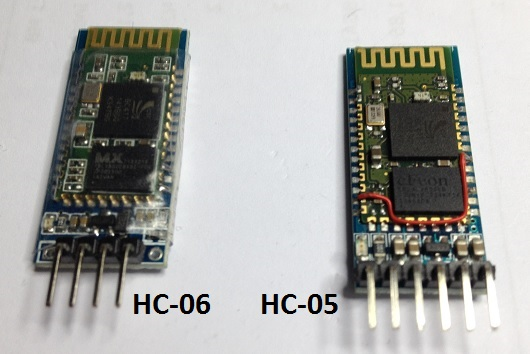
\includegraphics[width=0.3\paperwidth]{images/bt-hc-06-vs-hc-05.jpg}
\caption{Módulos Bluetooth HC-06 vs HC-05}
\footnotesize
Fuente: www.prometec.net $\mid$ MÓDULO BLUETOOTH HC-06. Under fair use. \cite{prometecnet-2019}
\end{figure}

\subsection{Programa que lee y escribe por Bluetooth}

El siguiente programa utiliza la librería $SoftwareSerial$ para establecer la conexión con el módulo Bluetooth HC-06 mediante Serial y según especificación a una velocidad de datos de $9,600 \, baudios$ la cual debe estar correctamente configurada. Recordar que las terminales $0$ y $1$ del Arduino están destinadas para la comunicación serial con el ordenador de acuerdo a artículos anteriores, por lo que se utilizarán otras terminales para el módulo Bluetooth.

\begin{lstlisting}[language=C, caption=Programa que lee y escribe por Bluetooth. Fuente: www.prometec.net $\mid$ MÓDULO BLUETOOTH HC-06. Under fair use. \cite{prometecnet-2019}]
// By https://www.prometec.net/bt-hc06/

#include <SoftwareSerial.h>

SoftwareSerial BT1(4,2);

void setup()
{
Serial.begin(9600);
Serial.println("Enter AT commands:");
BT1.begin(9600);
}

void loop()
{
if (BT1.available())
{
Serial.write(BT1.read());
}
if (Serial.available())
{
String str = getLine();
BT1.print(str);
Serial.println("---> " + str);
}
}

String getLine()
{
String S = "" ;
if (Serial.available())
{
char c = Serial.read();
while (c != '\n')
{
S = S + c;
delay(25);
c = Serial.read();
}
return(S + '\n');
}
}
\end{lstlisting}

\bigbreak

Como se explicó, se importa la librería $SoftwareSerial$ para crear un objeto $BT1$ el cual nos da el API para comunicarse con el dispositivo Bluetooth. Así mismo, el serial del Arduino se usa para comunicarse con el ordenador. En el loop se ve que al existir datos del dispositivo bluetooth se leen e imprimen por el serial, y si hay datos esperando en el serial entonces se solicita una línea de texto a ingresar para posteriormente mandarla por el dispositivo Bluetooth.

\bigbreak

Para leer la línea de texto del serial, se concatena el string mediante la entrada de $Serial.read()$ hasta que se ingrese una nueva línea o enter en el ordenador.

El circuito es trivial y se ilustra a continuación.

\begin{figure}[H]
\centering
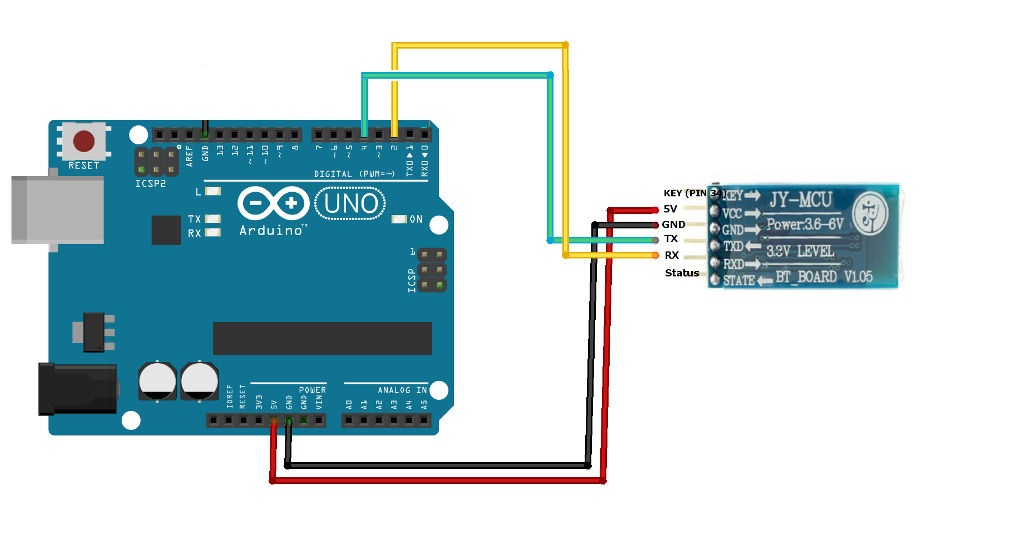
\includegraphics[width=0.3\paperwidth]{images/bt-arduino-circuit.jpg}
\caption{Circuito para conexión de Arduino con módulo Bluetooth HC-06}
\footnotesize
Fuente: www.prometec.net $\mid$ MÓDULO BLUETOOTH HC-06. Under fair use. \cite{prometecnet-2019}
\end{figure}

Para probar la otra parte del sistema, se puede utilizar un smartphone con alguna aplicación como Bluetooth SPP Manager para establecer la comunicación con el módulo Bluetooth HC-06.

\section{Motor DC}

Los motores de corriente directa fueron de los primeros en usarse ampliamente y transforman la energía eléctrica en mecánica. Su funcionamiento está relacionado con torques, bobinas y electromagnetismo.

\subsection{Control de un Motor DC con PWM}

El motor se controlará mediante salida análogo con PWM. Recordar que PWN modula la señal que se envía para controlar la potencia entregada al hacer variar el ancho de la onda cuadrada o digital lo cual hace un promedio de voltaje entregado en cada ciclo por lo cual la potencia que es proporcional al voltaje es eventualmente controlada.

\bigbreak

El código es el siguiente:

\begin{lstlisting}[language=C, caption=Control de motor DC con PWM. Fuente: Adafruit Learning System $\mid$ Arduino Lesson 13. DC Motors. Under fair use. \cite{monk-dc-motors-2012}]
/*
Adafruit Arduino - Lesson 13. DC Motor
*/

int motorPin = 3;

void setup()
{
pinMode(motorPin, OUTPUT);
Serial.begin(9600);
while (!Serial);
Serial.println("Speed 0 to 255");
}

void loop()
{
if (Serial.available())
{
int speed = Serial.parseInt();
if (speed >= 0 && speed <= 255)
{
analogWrite(motorPin, speed);
}
}
}
\end{lstlisting}

Se define la terminal para el motor como la $3$ en modo salida. En el loop se lee el valor en $[0, 255]$ del Serial para controlar la velocidad del motor. Este valor se escribe mediante PWM y el método $analogWrite$.

\bigbreak

El diagrama contiene algunos aspectos a tener en cuenta:

\begin{figure}[H]
\centering
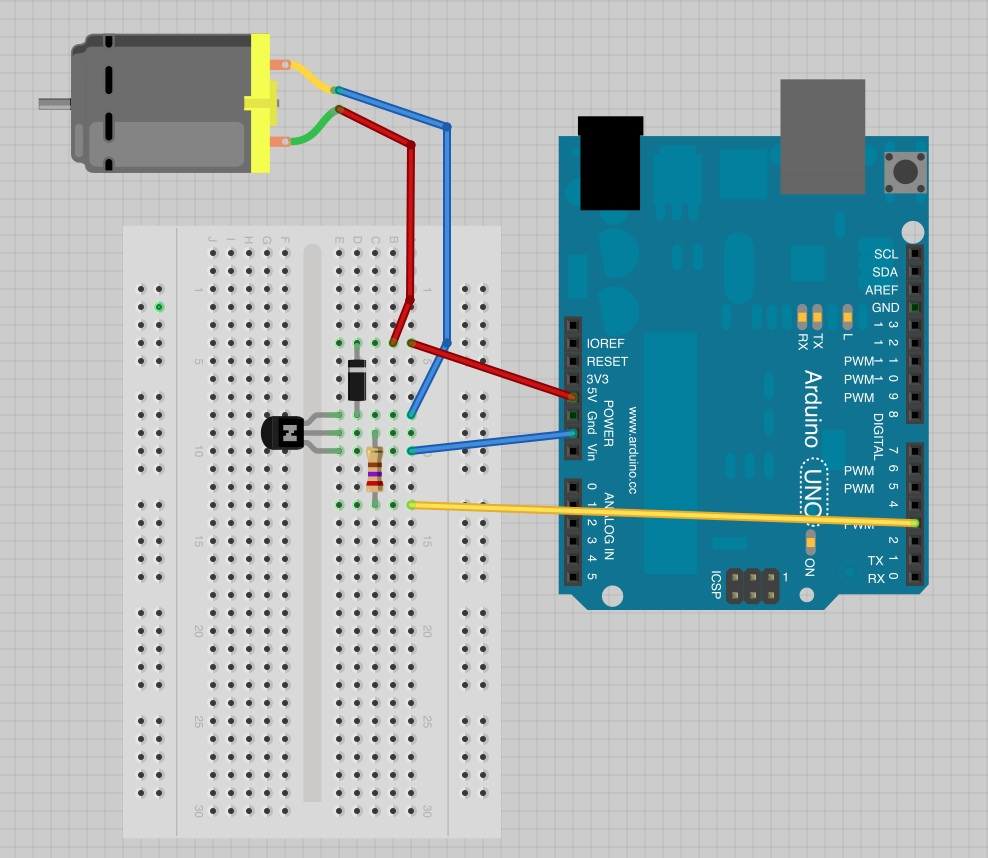
\includegraphics[width=0.3\paperwidth]{images/dc-motor-arduino-circuit.jpg}
\caption{Circuito para control de motor DC en Arduino}
\footnotesize
Fuente: Adafruit Learning System $\mid$ Arduino Lesson 13. DC Motors. By Simon Monk. Licensed under the Attribution Creative Commons License.
\end{figure}

Aquí vemos que se requiere:

\begin{itemize}
\item 1 Motor DC 6V
\item 1 Transistor PN2222
\item 1 Diodo 1N4001
\item 1 Resistencia $270 \Omega$
\item Tarjeta Arduino
\item Otros como cables
\end{itemize}

\bigbreak

El transistor actúa como conmutador para controlar el motor con la señal que recibe en su base desde el pin del Arduino y hacia el colector que conecta al motor mediante el diodo y el emisor que va a tierra. Notar que, como usualmente cuando se estudia electrónica, ponemos un diodo cuando hay dispositivos inductivos como bobinas o motores para evitar una descarga con corriente en dirección opuesta hacia nuestro circuito o polarizaciones incorrectas. También, el motor consume mucha corriente obviamente por lo que el Arduino no lo puede manejar, y se usa un simple transistor para el control de potencia.

\section{Conclusión}


\printbibliography

\end{document}
